\documentclass[12pt, a4paper, oneside]{ctexart}
\usepackage{amsmath, amsthm, amssymb, graphicx}
\usepackage{hyperref}
\usepackage{listings}
\usepackage{xcolor}
\usepackage{color}
\usepackage{enumerate}
\usepackage{epstopdf}
\usepackage{float}
\usepackage{framed}
\usepackage{titlesec}
\usepackage{cite}
\usepackage{booktabs}
\usepackage{geometry}
\usepackage{caption}
\usepackage{subfigure}
\usepackage[section]{placeins}
\usepackage{fancyhdr}%导入fancyhdr包
\usepackage{ctex}%导入ctex包
\usepackage[ruled,vlined]{algorithm2e}
\hypersetup{
    colorlinks=true,
    linkcolor=blue,
    filecolor=blue,      
    urlcolor=blue,
    citecolor=cyan,
}
\definecolor{dkgreen}{rgb}{0,0.6,0}
\definecolor{gray}{rgb}{0.5,0.5,0.5}
\definecolor{mauve}{rgb}{0.58,0,0.82}
\definecolor{shadecolor}{rgb}{0.5,0.5,0.5}
\lstset{ %
    language=Python,                % the language of the code
    basicstyle=\footnotesize,           % the size of the fonts that are used for the code
    numbers=left,                   % where to put the line-numbers
    %numberstyle=\tiny\color{gray},  % the style that is used for the line-numbers
    %stepnumber=2,                   % the step between two line-numbers. If it's 1, each line 
                            % will be numbered
    %numbersep=5pt,                  % how far the line-numbers are from the code
    %backgroundcolor=\color{blue},      % choose the background color. You must add \usepackage{color}
    showspaces=false,               % show spaces adding particular underscores
    %showstringspaces=false,         % underline spaces within strings
    showtabs=false,                 % show tabs within strings adding particular underscores
    frame=single,                   % adds a frame around the code
    rulecolor=\color{black},        % if not set, the frame-color may be changed on line-breaks within not-black text (e.g. commens (green here))
    tabsize=2,                      % sets default tabsize to 2 spaces
    captionpos=b,                   % sets the caption-position to bottom
    breaklines=true,                % sets automatic line breaking
    breakatwhitespace=false,        % sets if automatic breaks should only happen at whitespace
    % title=\lstname,                   % show the filename of files included with \lstinputlisting;
                            % also try caption instead of title
    keywordstyle=\color{blue},          % keyword style
    commentstyle=\color{dkgreen},       % comment style
    stringstyle=\color{mauve},         % string literal style
    escapeinside={\%*}{*)},            % if you want to add LaTeX within your code
    morekeywords={*,...}               % if you want to add more keywords to the set
}
\title{数据分析及实践\_Assignment3}
\author{Xiaoma}
\date{\today}
\pagestyle{fancy}

\lhead{第 3 次实验\\\today}
\chead{中国科学技术大学\\数据分析及实践}

\rhead{Assignment 3\\ {\CTEXoptions[today=old]\today}}
\newcommand{\upcite}[1]{\textsuperscript{\cite{#1}}}
\begin{document}
\maketitle
\section{实验要求}
\begin{itemize}
    \item 基于筛减版的\textbf{PISA}数据集,进行数据分析、统计以及抽取特征
    \item 数据分析统计如\begin{itemize}
        \item 单个特征的分布
        \item 统计缺失值
        \item 特征间的相关性
        \item 推测特征的含义
        \item 异常样本
    
    \end{itemize}
    \item 特征抽取如\begin{itemize}
        \item 特征的变换
        \item 尝试组合特征
        \item 特征子集选择
    \end{itemize}
\end{itemize}

\newpage
\section{实验环境}
\textbf{VSCode + Python3.9.13}
\section{实验步骤}
\subsection{数据清洗}
\subsubsection{初步筛选特征}
读取全部数据,并查看数据信息。该数据集共有487个特征,42176条数据。

首先丢弃数据集中无意义的特征
\begin{itemize}
    \item 索引特征:Unnamed:0与index
    \item 值唯一的特征:ADMINMODE与LANGTEST\_COG
\end{itemize}

统计数据集中每个特征的缺失值数量,综合数据量以及特征量,将缺失值比率超过0.1的特征从数据集中丢弃,最终得到的
特征数量为179个。

对照特征名与\textbf{codebook}表来推测每个特征对应的含义,通过比较发现,特征CNTRYID与CNT,NatCen意义重复,
故丢弃特征CNT,NatCen。特征STRATUM,SUBNATIO的地域信息更为详细,但数据过于复杂,故也被丢弃。

查看剩余特征的数据类型,均为\textbf{int}或\textbf{float},故不需要进行数据类型转换。

\subsubsection{缺失值处理}

计算数据集中每个特征的方差,发现特征的方差均较小,综合数据量以及特征量,使用均值填充缺失值。

\subsection{特征选择}

\subsubsection{基于嵌入法进行特征选择}
分别基于\textbf{XGBClassifier,LGBMClassifier,DecisionTree}对数据进行训练后,比较每个特征在预测过程中的重要性
占比,可视化根据特征的预测过程,选择与预测任务最相关的若干特征绘制pearson相关系数热力图。
\begin{figure*}[htbp]
    \centering
	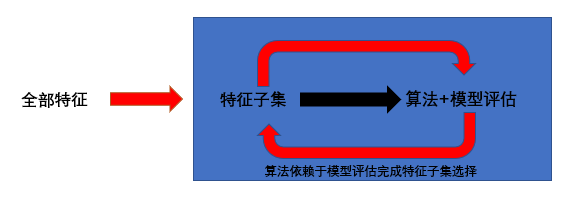
\includegraphics[width=1\textwidth]{./img/14.png}
\end{figure*}
特征重要性以及预测过程分别如图所示
\begin{figure}[h!]
    \subfigure[$XGBoost\_FeatureImportance$]{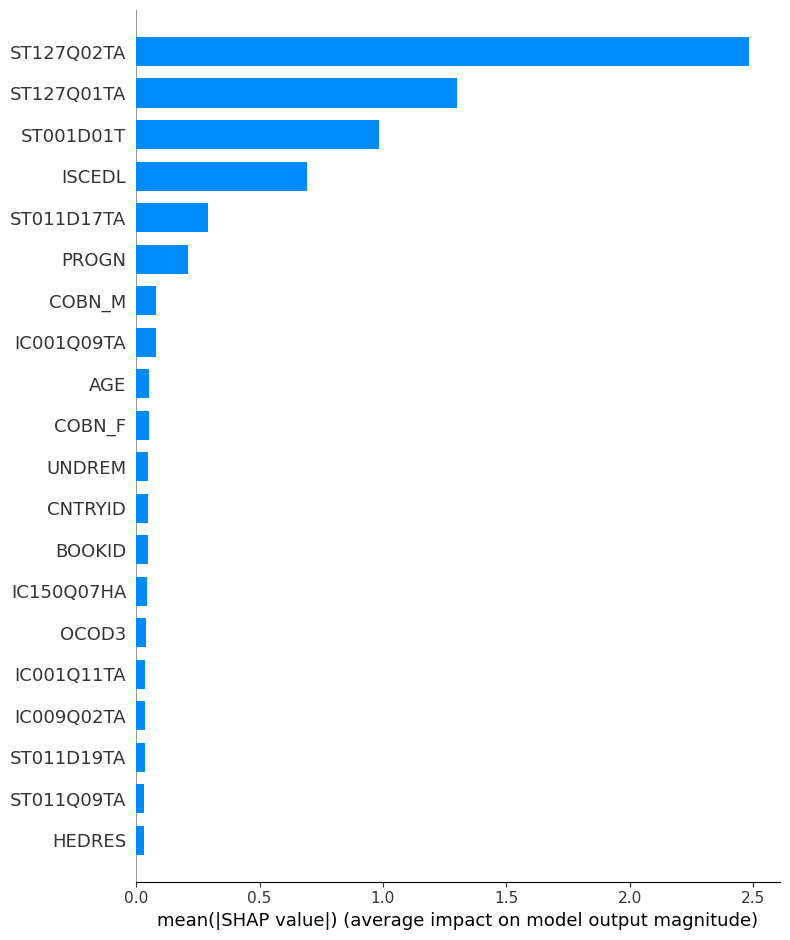
\includegraphics[width=0.45\hsize]{./img/1.png}} 
    \subfigure[$XGBoost\_PredictProcess$]{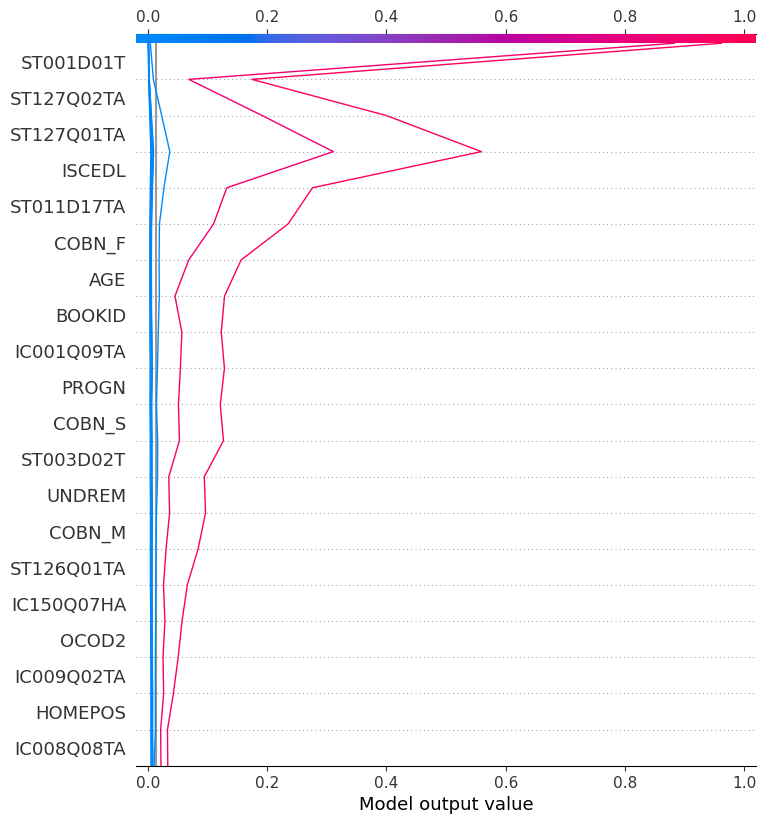
\includegraphics[width=0.45\hsize]{./img/3.png}}\\
    \label{wildlife}
\end{figure}
\begin{figure}[h!]
    \subfigure[$XGBoost\_FeatureImportance$]{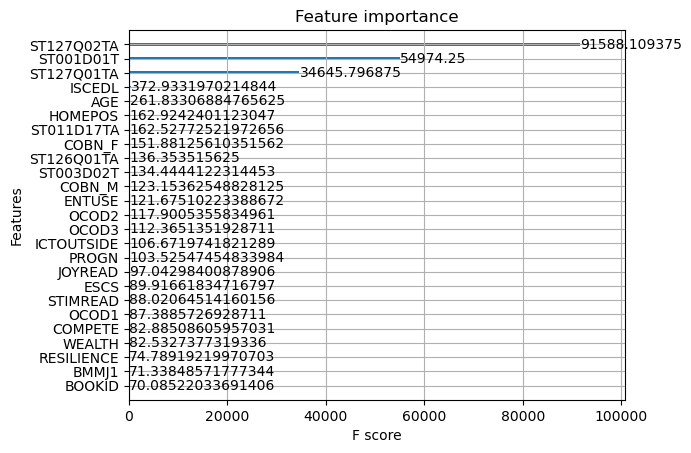
\includegraphics[width=0.45\hsize]{./img/2.png}} 
    \subfigure[$XGBoost\_HeatMap$]{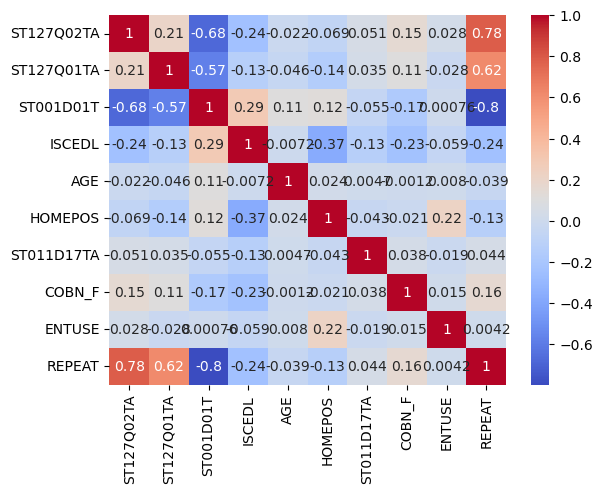
\includegraphics[width=0.45\hsize]{./img/4.png}}\\
    \label{wildlife}
\end{figure}
\begin{figure}[h!]
    \subfigure[$LGBM\_FeatureImportance$]{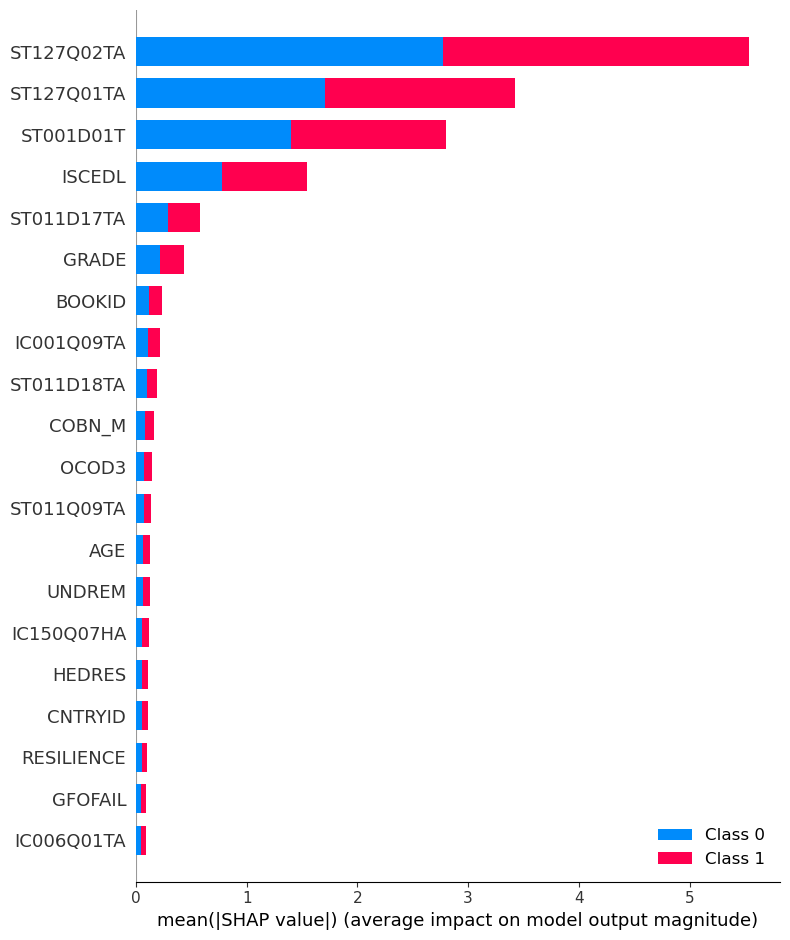
\includegraphics[width=0.45\hsize]{./img/5.png}} 
    \subfigure[$LGBM\_PredictProcess$]{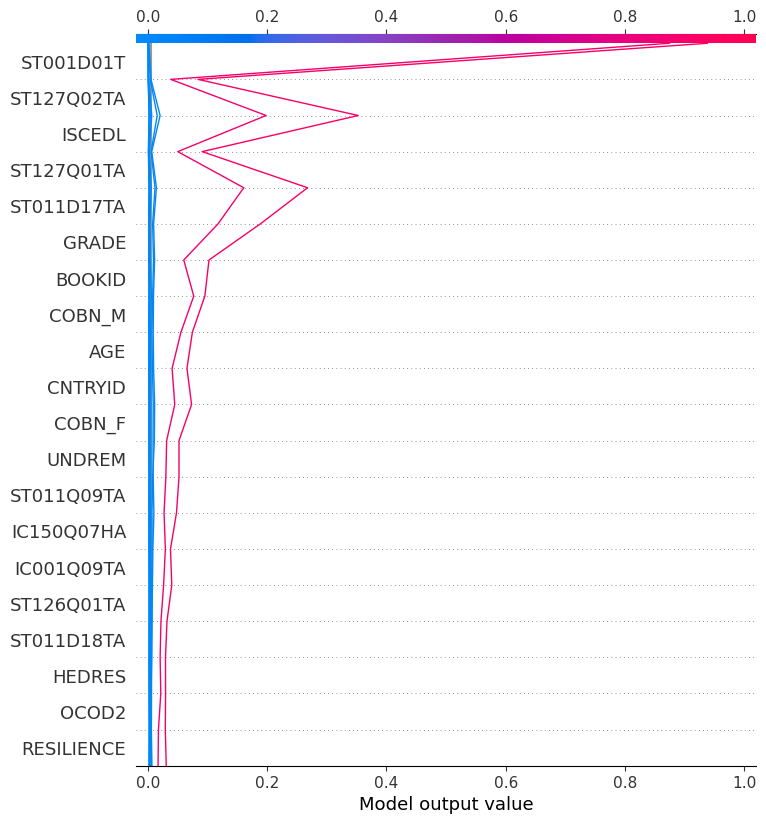
\includegraphics[width=0.45\hsize]{./img/7.png}}\\
    \label{wildlife}
\end{figure}
\begin{figure}[h!]
    \subfigure[$LGBM\_FeatureImportance$]{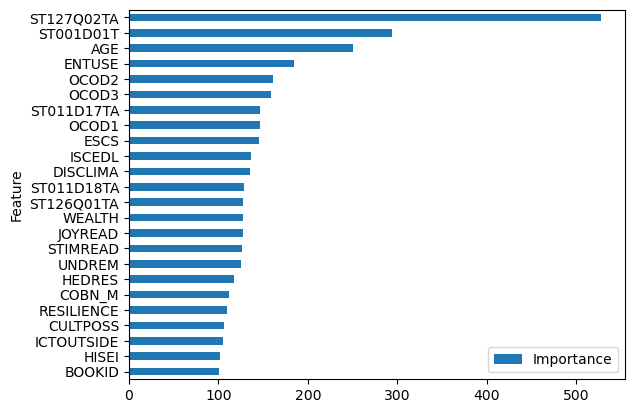
\includegraphics[width=0.45\hsize]{./img/6.png}} 
    \subfigure[$LGBM\_HeatMap$]{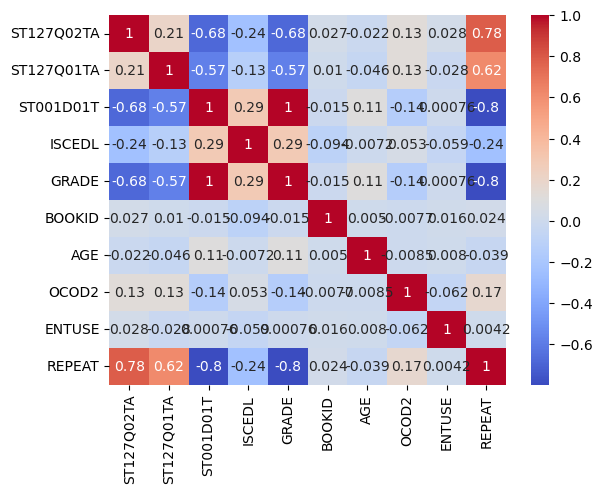
\includegraphics[width=0.45\hsize]{./img/8.png}}\\
    \label{wildlife}
\end{figure}
\begin{figure}[h!]
    \subfigure[$DecisionTree\_FeatureImportance$]{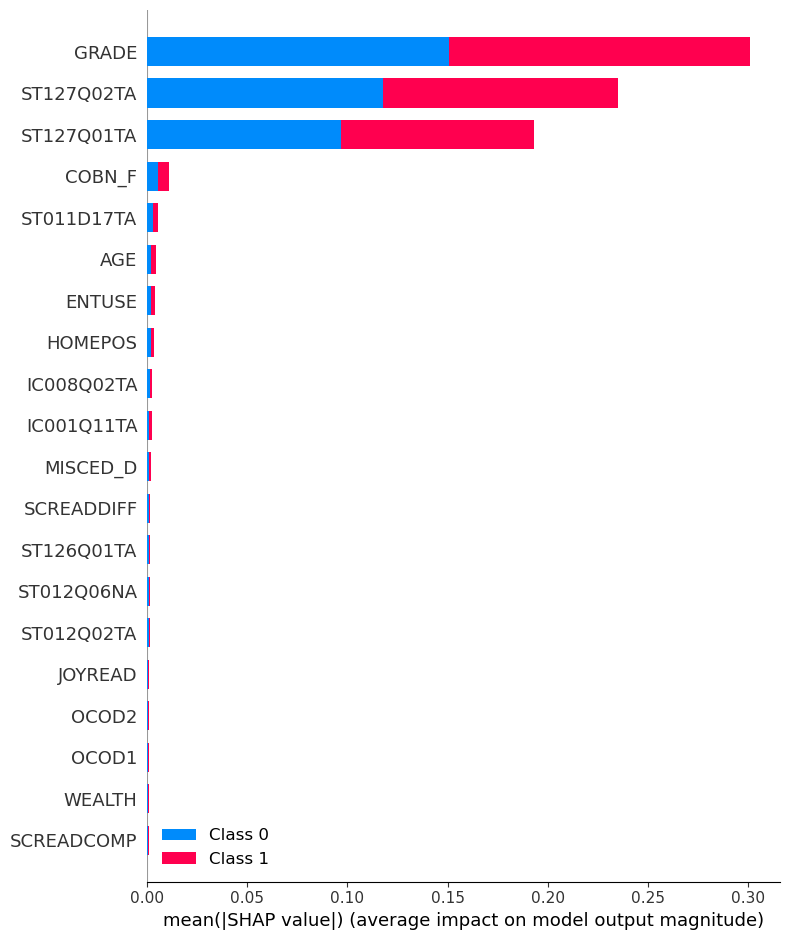
\includegraphics[width=0.45\hsize]{./img/9.png}} 
    \subfigure[$DecisionTree\_PredictProcess$]{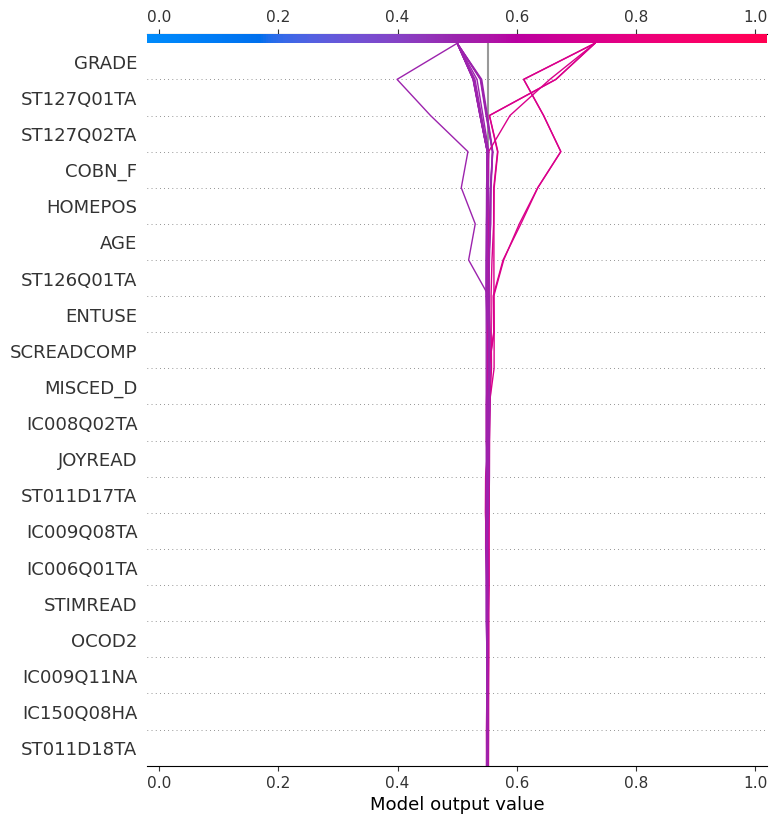
\includegraphics[width=0.45\hsize]{./img/11.png}}\\
    \label{wildlife}
\end{figure}
\begin{figure}[h!]
    \subfigure[$DecisionTree\_FeatureImportance$]{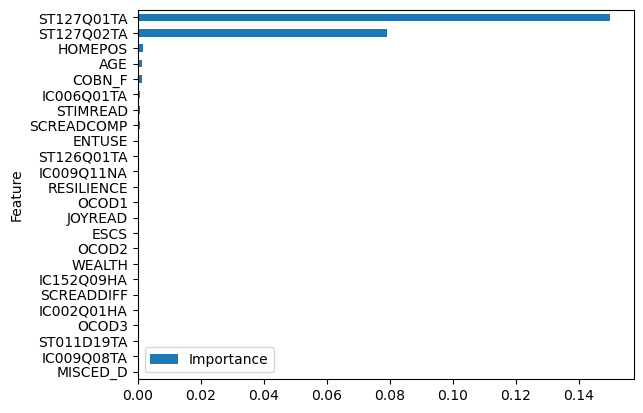
\includegraphics[width=0.45\hsize]{./img/10.png}} 
    \subfigure[$DecisionTree\_HeatMap$]{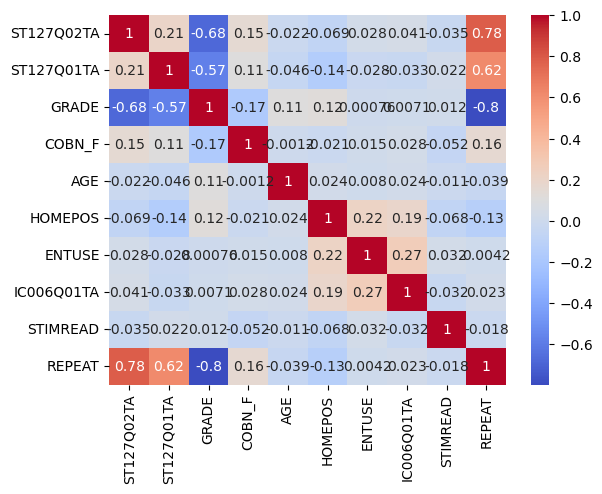
\includegraphics[width=0.45\hsize]{./img/12.png}}\\
    \label{wildlife}
\end{figure}

\clearpage
综合上述模型对应的特征重要性,最终选择\textbf{ST127Q02TA,ST127Q01TA,\\ST001D01T,GRADE,COBN\_F,HOMEPOS,ISCEDL,OCOD2}   作为\textbf{REPEAT}预测任务的训练特征。




\subsection{相关性分析}
所选择的8个特征与\textbf{REPEAT}的pearson相关系数为
\begin{figure*}[htbp]
    \centering
	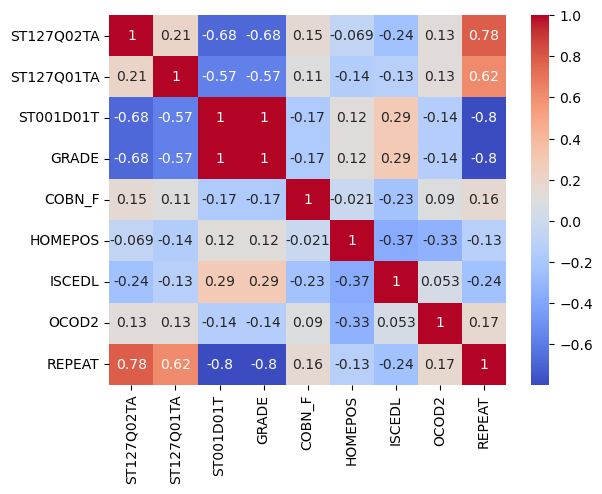
\includegraphics[width=1\textwidth]{./img/13.png}
\end{figure*}


分别使用\textbf{XGBoost,DecisionTree}对数据进行训练,10折交叉验证的正确率分别为\textbf{0.997,0.993},与未进行数据筛选前精度几乎不变,
意味着所选择的8个特征为参与预测任务的主要特征,丢弃其他特征对预测任务几乎无影响。

查询所选的8个特征对应的意义,并观察其值的分布规律。

通过查询\textbf{codebook}表,特征对应的意义分别为
\begin{table*}[t]
    \centering%把表居中
    \begin{tabular}{cc}%内容全部居中
    \toprule%第一道横线
    特征名&含义 \\
    \midrule%第二道横线 
    \textbf{ST127Q02TA} &Have you ever repeated a <grade>? At <ISCED 2>\\
    \textbf{ST127Q01TA} &Have you ever repeated a <grade>? At <ISCED 1>\\
    \textbf{ST001D01T} &Student International Grade (Derived)\\
    \textbf{GRADE} & Grade compared to modal grade in country\\
    \textbf{COBN\_F} &Country of Birth National Categories- Father\\
    \textbf{HOMEPOS} &Home possessions (WLE)\\
    \textbf{ISCEDL} & ISCED level\\
    \textbf{OCOD2} & ISCO-08 Occupation code - Father\\

    \bottomrule%第三道横线
    \end{tabular}
\end{table*}
\section{总结}
通过上述特征选择的过程,发现所选择的8个特征为预测\textbf{REPEAT}标签的重要特征,
并且通过分析特征对应的含义发现,部分特征与预测任务的关系,根据生活经验仍可以判断具有强强相关
性,并通过这些特征来发现剩余特征与预测任务的新的关系,说明本次特征选择是有意义且正确的。

\end{document}